\section{Radds存储系统部署、日志分析与测试}

	\subsection{存储系统部署}

	\begin{enumerate}
		
		\item 选择合适的硬件机器 
		
		由于Golang语言跨平台的特性,本文选择的文件系统操作方案也具有跨平台的特性,所以Radds存储系统具有跨平台的特点。

		
		\item 下载相应平台上的Golang编译器 
		
		在Golang官网上下载相应机器架构,相应操作系统的Golang编译器

		\item 编译源代码工程文件
		
		对本文写好的源代码工程文件进行编译,和自动化测试

	\end{enumerate}



	\subsection{存储系统客户端测试}
	

	进入命令行客户端后,输入命令
	
	\begin{enumerate}
		
		\item 命令行命令概览
		
		下图是命令行客户端的命令总体概览
		\begin{figure}[H]
			\centering
			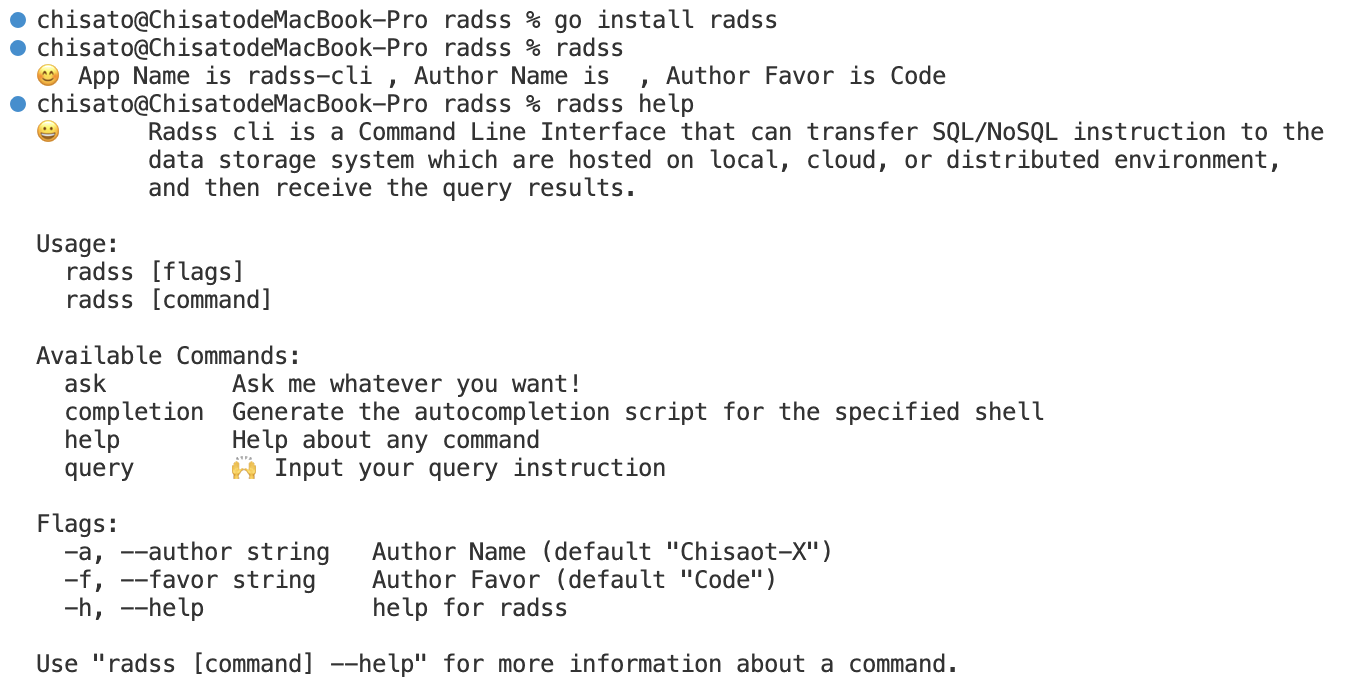
\includegraphics[width=0.95\textwidth]{images/radds_cli_all.png}
			\caption{命令行客户端命令总体概览}
			\label{cli_overall}
		\end{figure}

		\item 命令行查询命令概览 
		
		下图是命令行客户端的查询命令概览
		\begin{figure}[H]
			\centering
			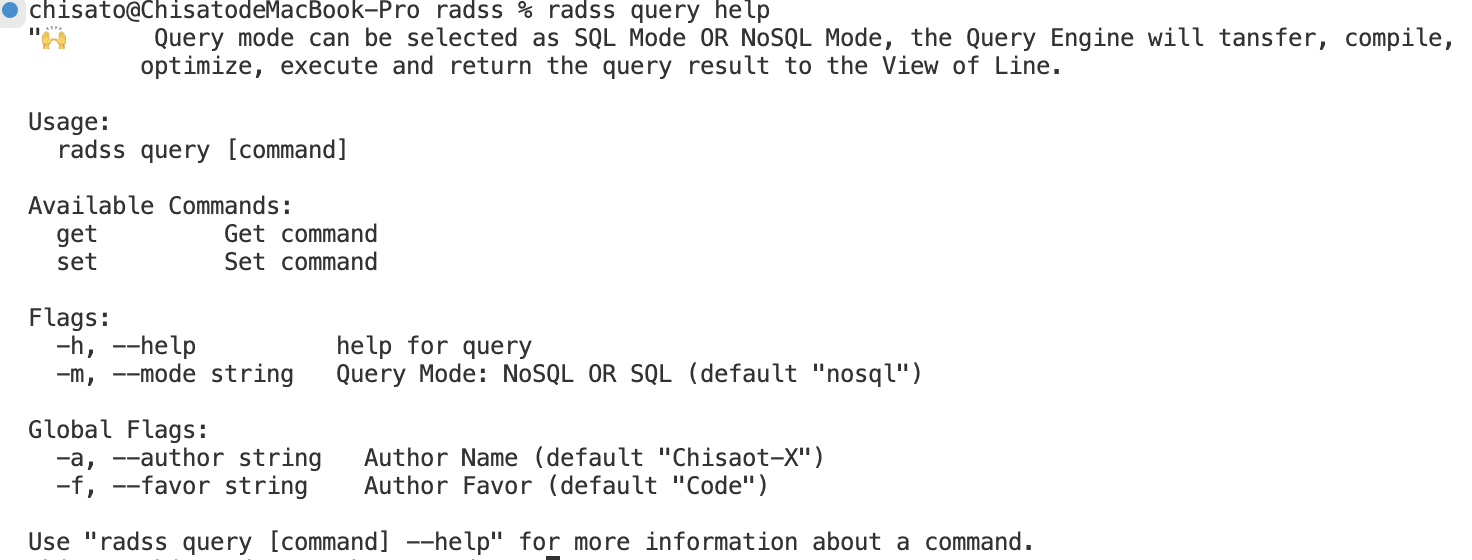
\includegraphics[width=0.95\textwidth]{images/radds_query_all.png}
			\caption{命令行客户端查询命令概览}
			\label{cli_query_overall}
		\end{figure}
		
		\item 命令行操作数据
		
		下图是如何使用命令行客户端操作数据的方法
		\begin{figure}[H]
			\centering
			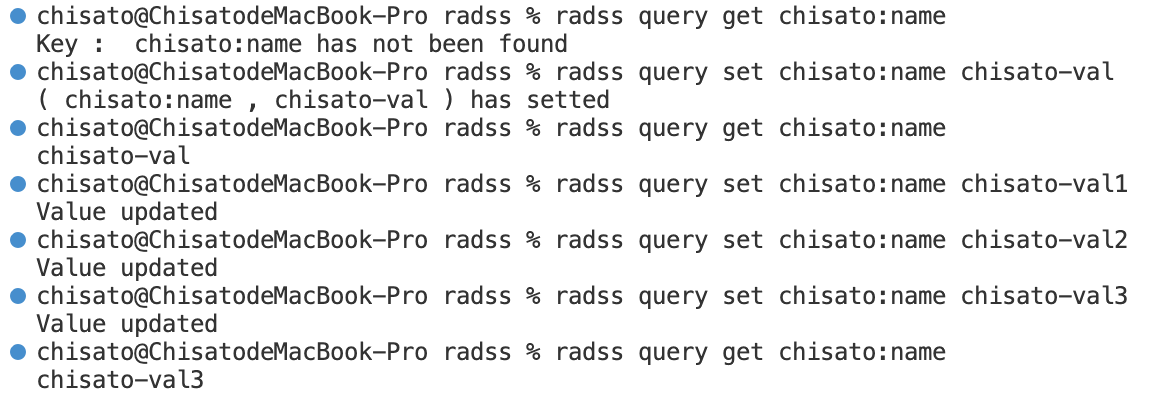
\includegraphics[width=0.95\textwidth]{images/radds_query.png}
			\caption{命令行操作数据}
			\label{cli_query}
		\end{figure}

	\end{enumerate}

	\subsection{存储系统日志分析}
	
	本文针对此存储系统的键值型存储方案,文件压缩方法,日志复制过程做日志分析。

	如图是配置文件的一个示例图,可以针对不同操作系统做变形
	\begin{figure}[H]
		\centering
		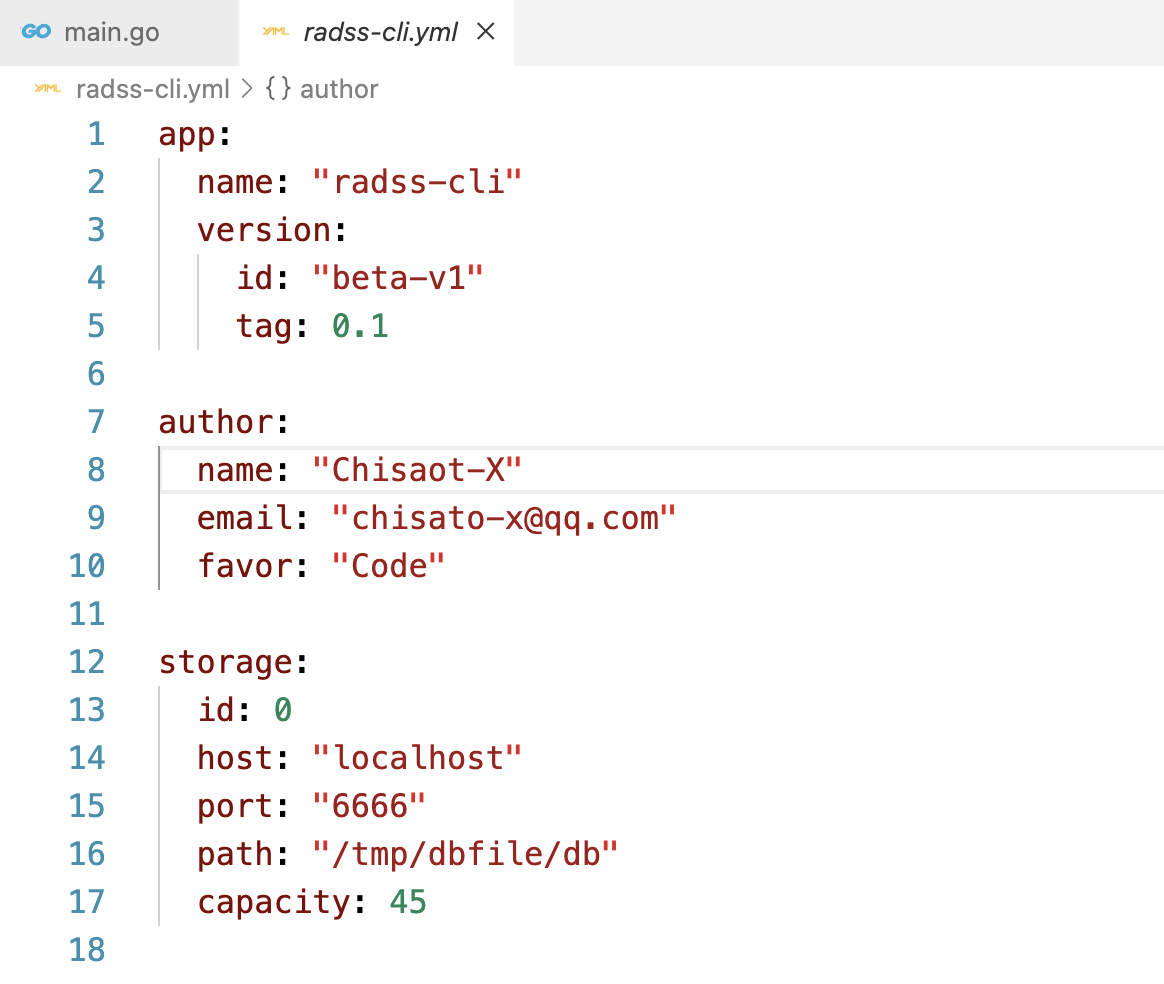
\includegraphics[width=0.95\textwidth]{images/radds_config.png}
		\caption{存储系统配置文件}
		\label{radds_config}
	\end{figure}

	本文进入操作系统的文件存储目录,打开日志文件:LOG

	\begin{figure}[H]
		\centering
		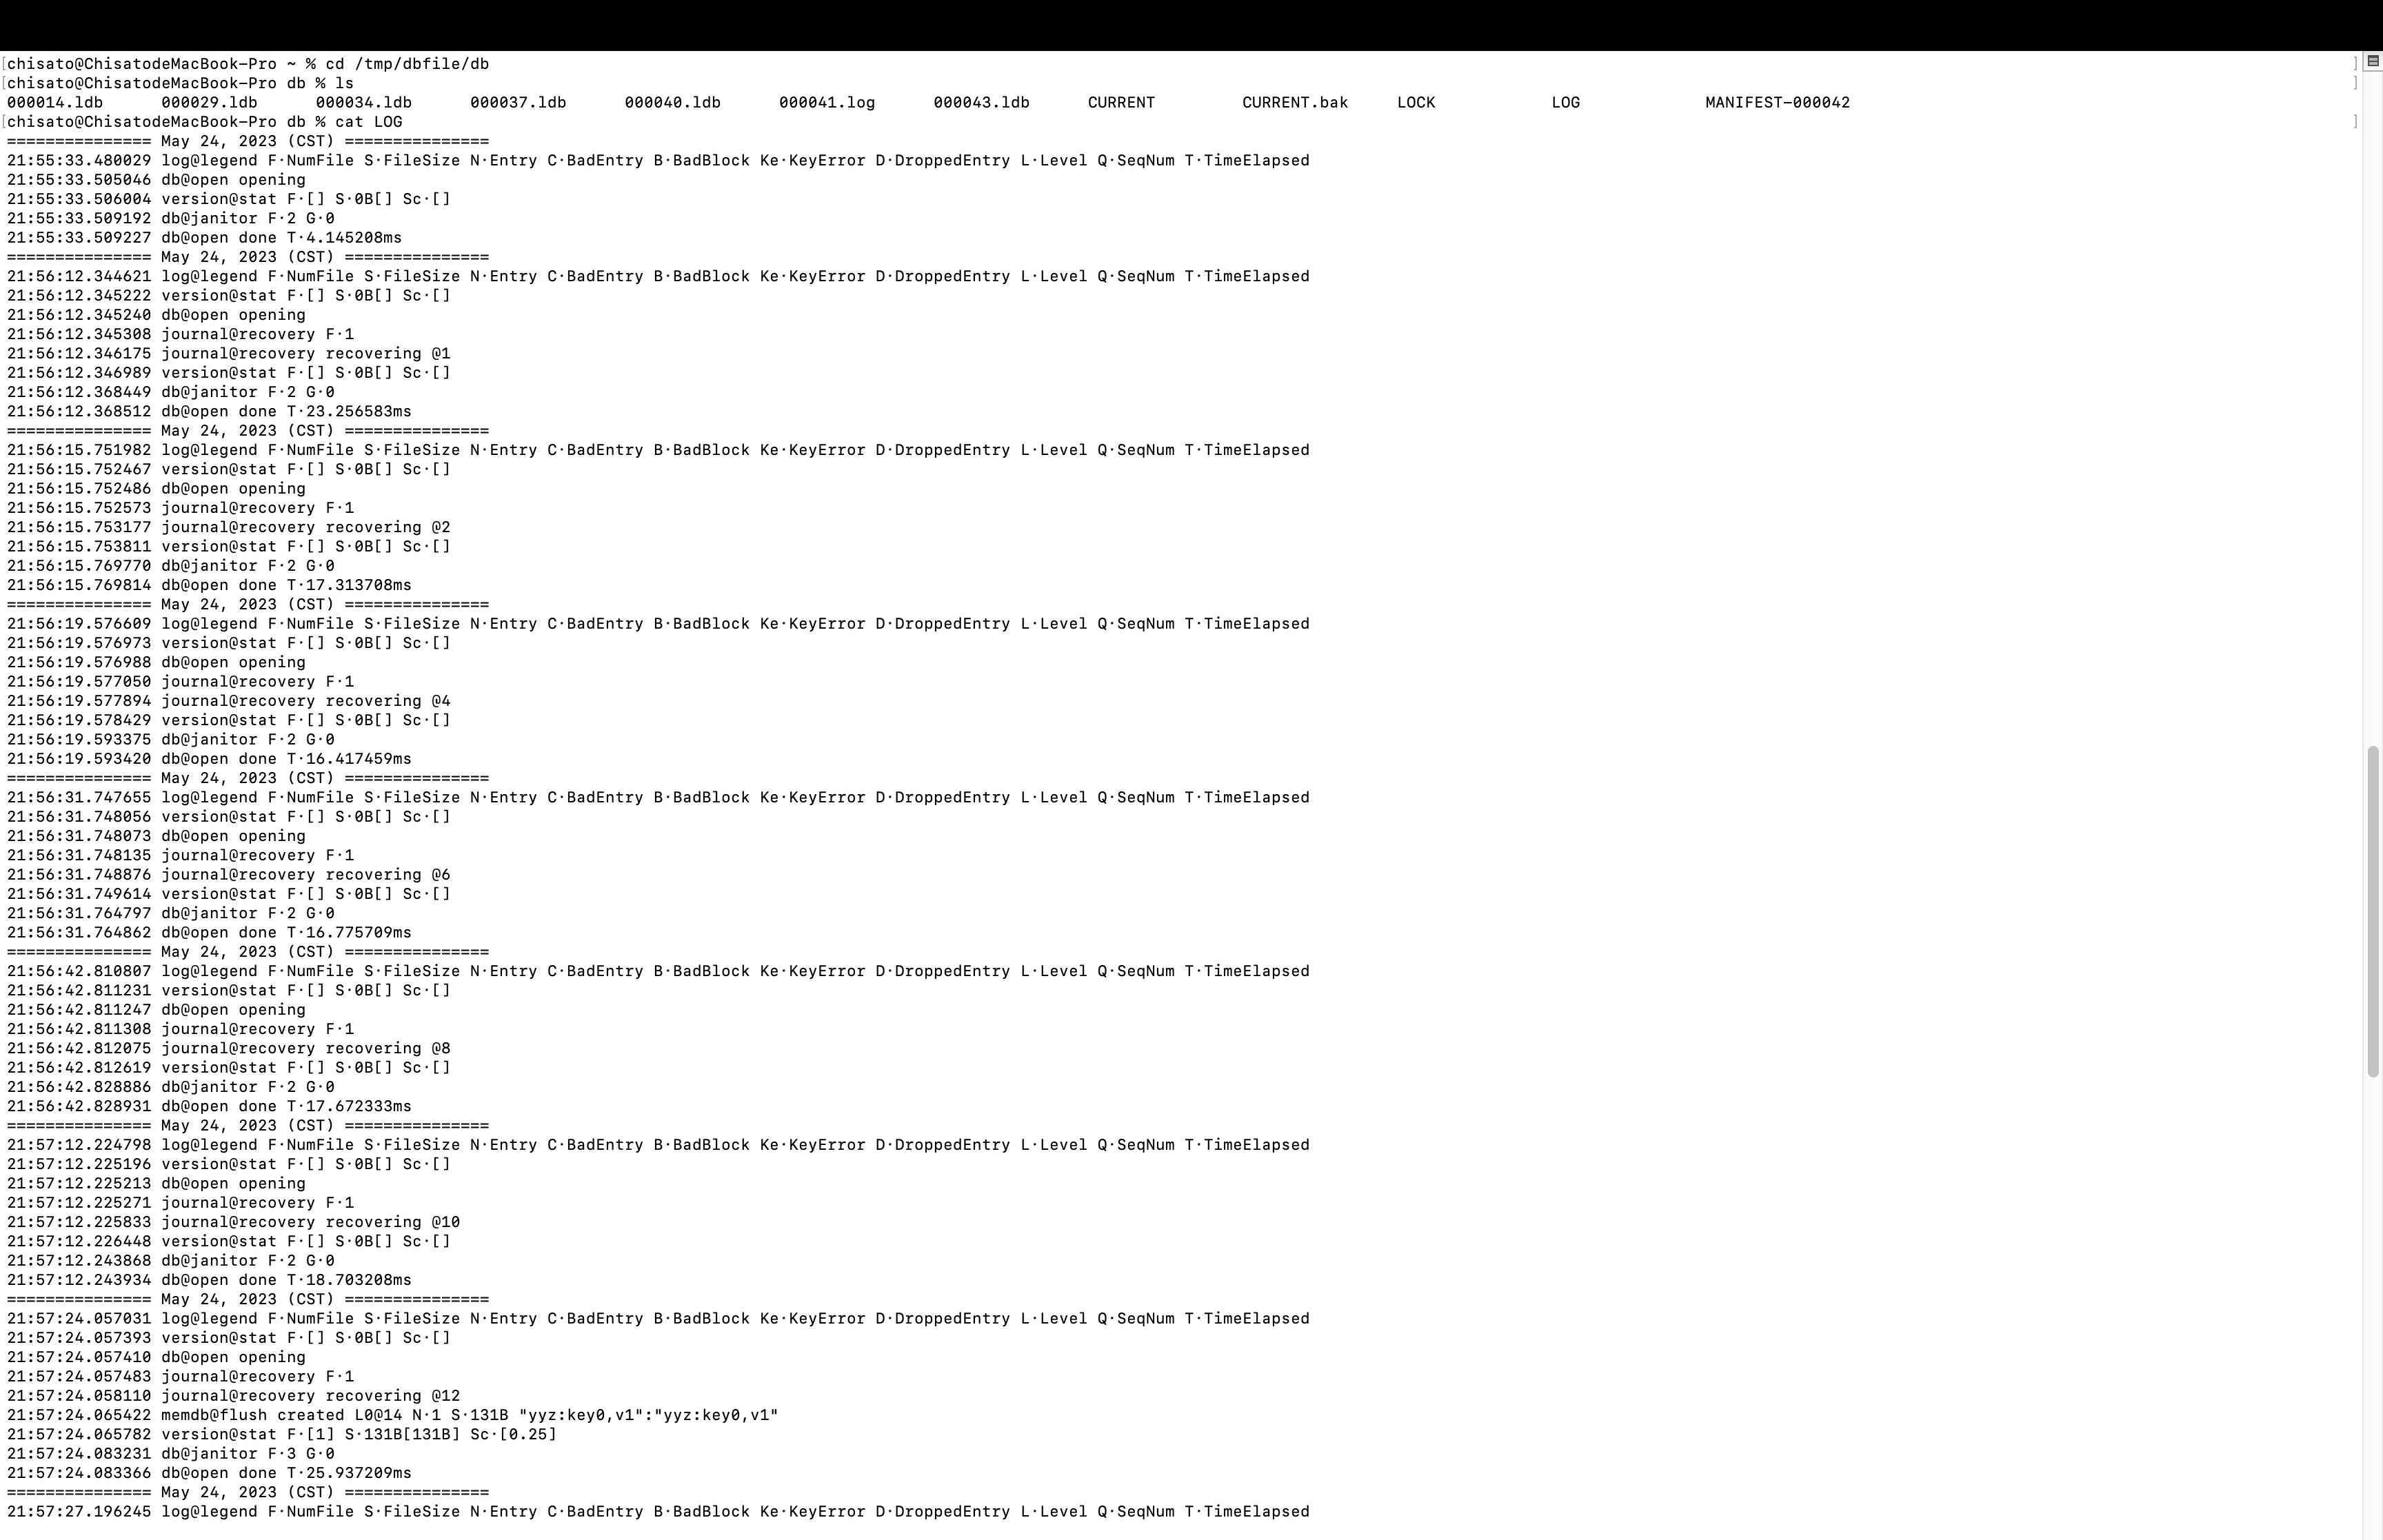
\includegraphics[width=0.95\textwidth]{images/radds_log.png}
		\caption{存储系统日志分析}
		\label{radds_log}
	\end{figure}

	将上述日志转换为表格:

	\begin{table}[h!]
		\centering
		\begin{tabular}{|c|c|}
		\hline
		操作类型 & 次数 \\
		\hline
		open & 10 \\
		\hline
		recovery & 10 \\
		\hline
		flush & 5 \\
		\hline
		janitor & 10 \\
		\hline
		compaction & 2 \\
		\hline
		\end{tabular}
		\caption{数据库操作的次数}
		\label{tab:db}
	\end{table}
		
		




	% \subsection{本章小结}
	
\clearpage